%Made By Thomas Debelle
\documentclass{report}
\usepackage[a4paper, total={6in, 9in}]{geometry}
\usepackage[utf8]{inputenc}
\usepackage[francais]{babel}
\usepackage{graphicx}
\usepackage{graphics}
\usepackage[T1]{fontenc}
\usepackage{amsmath}
\usepackage{hyperref}
\usepackage{amssymb}
\usepackage{listings}
\usepackage{xcolor}
\usepackage{color}
\usepackage{array}
\usepackage{float}
\usepackage{amsfonts}
\usepackage{fancyhdr}
\usepackage{titlesec}
\usepackage{xparse}

\hypersetup{
    colorlinks=true,
    linkcolor=black,
    filecolor=magenta,
    urlcolor=cyan,
    pdftitle={Overleaf Example},
    pdfpagemode=FullScreen,
    }
\begin{document}


\begin{titlepage}
    \begin{figure}
        
\includegraphics[height = 2cm]{Images/Template/UCL_Logo.png}
        \label{fig:my_label}
    \end{figure}

    \hspace*{100cm}
    \centering
    \vspace*{7cm}

    {\Huge \textbf{Résumé de LMECA1210 - DAM}}\\
    \vspace*{0.25cm}
    compilation du \today\\
    \vspace*{0.25cm}
    \Large{Edouard Massart, Julien Monfils, \textbf{Ajoutez vos noms si vous participez}}\\

    \vspace*{9cm}
    {\Large Juin 2023}
\end{titlepage}


\tableofcontents
\newpage

\section*{Préface}

Bonjour à toi !\\

Cette synthèse recueille toutes les informations importantes données au cours, pendant les séances de tp et est améliorée grâce au note du Syllabus. Elle ne remplace pas le cours donc écoutez bien les conseils et potentielles astuces que les professeurs peuvent vous donner. Notre synthèse est plus une aide qui, on l'espère, vous sera à toutes et tous utile.\\

Elle a été réalisée par toutes les personnes que tu vois mentionnées. Si jamais cette synthèse a une faute, manque de précision, typo ou n'est pas à jour par rapport à la matière actuelle ou bien que tu veux simplement contribuer en y apportant tes connaissances ? Rien de plus simple ! Améliore la en te rendant \href{http://www.github.com/Tfloow/Q4_EPL}{ici} où tu trouveras toutes les infos pour mettre ce document à jour. (\textit{en plus tu auras ton nom en gros ici et sur la page du github})\\

Nous espérons que cette synthèse te sera utile d'une quelconque manière ! Bonne lecture et bonne étude.

\chapter{Introduction}

\chapter{Cinématique}
\section{Théorème d'Euler}
\subsection{Énoncé du théorème}
\textit{Tout déplacement d’un corps ayant un point fixe est une rotation autour d’un
axe — fixe — passant par ce point.} 
\footnote{Source : Syllabus, page 8}\\

\subsection{Démonstration}

Afin de monter cela, on va considérer une base inertielle $\left[ \hat{\textbf{I}}\right]$, ainsi que $\left[ \hat{\textbf{x}}\right]$, une seconde base intertielle telle que $\left[ \hat{\textbf{x}}\right] = \textbf{A} \left[ \hat{\textbf{I}}\right] $. Où $A$ est une matrice de rotation\\
On va montrer qu'il existe un vecteur $\hat{\textbf{e}}$ possédant les mêmes composantes dans les deux repères. C'est à dire 
\begin{align*}
    \hat{e} &= A\hat{e}\\
    \left( A - I\right) \hat{e} &= 0
\end{align*}
C'est un problème aux valeurs propres. Il nous faut alors montrer que la matrice $A$ possède une valeur propre $\lambda = 1$ avec pour vecteur propre $\hat{\textbf{e}}$.\\

Comme $A$ est une matrice de rotation, on sait que 
\begin{itemize}
    \item $det(A) = \lambda_1 \lambda_2 \lambda_3 = 1$
    \item $A = A^T \Rightarrow A^{-1}v_i = A^T v_i =(\lambda_i)^{-1} v_i$
    \item Les valeurs propres de $A^T$ sont les mêmes que celles de $A$
\end{itemize}
On en déduit que si $\lambda'$ est une valeur propre de $A$, alors $(\lambda')^{-1}$ l'est également.
\begin{equation*}
    det(A) = \lambda' (\lambda'^{-1}) \lambda* = \boxed{\lambda* = 1}
\end{equation*}
\section{Théorême de Chasles}
\subsection{Énoncé du théorême}

Ci-dessous vous trouvez le théorême de Chasles. Cependant, il nécessite deux notions intuitives à comprendre avant de pouvoir le démontrer : \\
\begin{itemize}
    \item La rotation successive autour de deux axes $a_i$ parallèles peut s'apparenter à une rotation autour d'un axe a parallèles aux axes $a_i$.
    \item Deux rotations succesives d'angle $\alpha$ et $-\alpha$ suivants des axes parallèles est en fait une translation ! En effet, en utilisant le principe énoncé plus haut, les deux rotations peuvent s'approximer par une rotation avec le centre a rejeté à l'infini ce qui nous donne un cercle de rayon infini. Un arc de cercle très petit est approximé par un segment de droite ce qui nous donne bien une translation !
\end{itemize}
\begin{figure}[H]
    \centering
    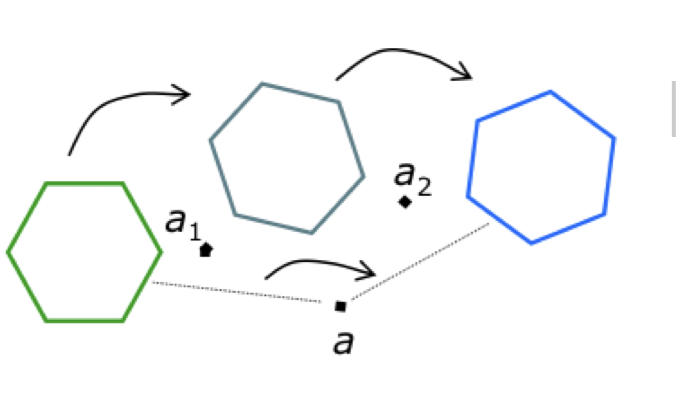
\includegraphics[width = 60 mm]{Images/imagesCinematique/Figure chasles 1.png}
    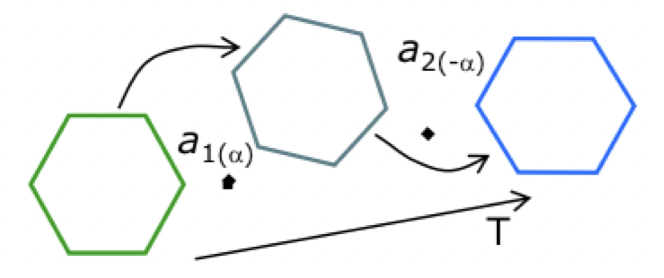
\includegraphics[width=60mm]
    {Images/imagesCinematique/Figure Chasles 2.png}
    \caption{Illustration du premier principe de Chasles}
    \label{fig:my_label}
\end{figure}
Nous pouvons donc grâce à ces deux principes énoncer le théorême de Chasles :\\

\textit{"Un déplacement fini quelconque d'un solide peut être représenté par la combinaison d'une translation et d'une rotation. Le mouvement ainsi est donc dit d'hélicoïdal."}

\section{Notions de glissement et de roulement}

\subsection{Point matériel et point géométrique}
On distingue deux types de point : 
\begin{itemize}
    \item Le point matériel, il est fixé sur un solide
    \item Le point géométrique, il n'est pas fixé et peut évoluer sur le solide au cours du temps
\end{itemize}

\section{Calcul du glissement et du roulement}

\subsection{Le glissement}

Attention, il faut faire la distinction entre glissement et frottement.
\begin{itemize}
    \item Le glissement : Vitesse relative (m/s) entre deux corps 
    \item Le frottement : Force (N) qui résulte du contact entre deux corps
\end{itemize}

\begin{figure}[H]
    \centering
    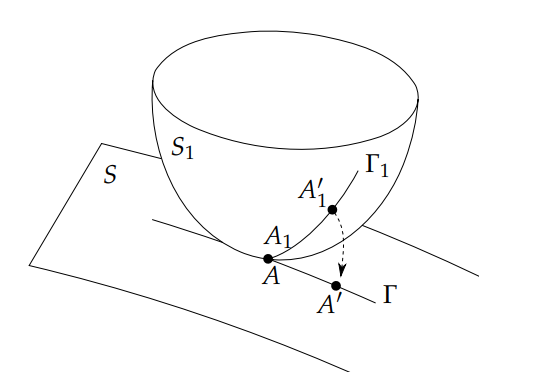
\includegraphics[width = 8cm]{Images/imagesCinematique/glissementg.png}
    \caption{bottom text}
    \label{fig:my_label}
\end{figure}
Pour comprendre ce qu'est le glissement, il faut imaginer deux coubres : 
\begin{itemize}
    \item $\Gamma$, la courbe composée de l'ensemble des points de contacts sur la surface immobile
    \item $\Gamma_1$, la courbe composée de l'ensemble des points de contacts sur le solide étudié.
\end{itemize}

On définira la vitesse de glissement $v_g$ comme la différence entre les vitesses de circulation des points de contact sur la courbe $\Gamma$ et $\Gamma_1$. En bref, c'est la vitesse relative entre la surface des deux solides en leur point de contact.

\subsection{Calculs du glissement, roulement et pivotement en pratique}


\begin{figure}[H]
    \centering
    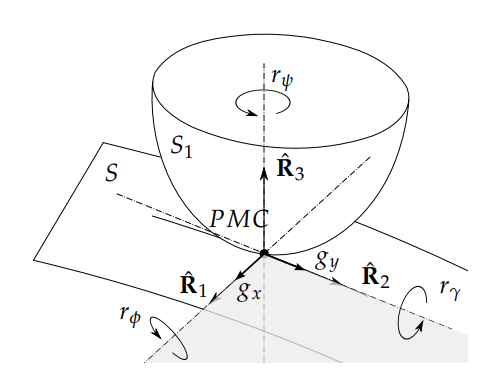
\includegraphics[width = 8cm]{Images/imagesCinematique/glissementRoulement.png}
    \label{fig:my_label}
\end{figure}

Pour calculer les glissements ($m/s$), il faut connaître la vitesse du PMC (point matériel de contact). Ensuite, il suffit de projeter cette vitesse dans le plan de contact.
\begin{align*}
    g_x &= \Vec{v}_{PMC} \cdot \hat{R}_1\\
    g_y &= \Vec{v}_{PMC} \cdot \hat{R}_2
\end{align*}

On trouve également les roulements ($rad/s$) avec les relations suivantes : 

\begin{align*}
    r_{\phi} &= \Vec{\omega}_{PMC} \cdot \hat{R}_1\\
    r_{\gamma} &= \Vec{\omega}_{PMC} \cdot \hat{R}_2\\
    r_{\psi} &= \Vec{\omega}_{PMC} \cdot \hat{R}_3
\end{align*}

\section{Mouvement général d'un solide}
\textcolor{red}{Je n'ai pas compris cette section donc je vous laisse l'écrire :-)\\
Je pense qu'il manque aussi la section sur les mouvements hélicoïdaux}

On a vu qu'un déplacement quelconque d'un solide peut être décomposé en
\begin{itemize}
    \item Une translation
    \item Une rotation parallèle à l'axe de translation.
\end{itemize}
C'est ce que l'on a appelé un déplacement hélicoïdale.\\
On va donc définir deux surfaces réglées : 
\begin{itemize}
    \item \textbf{L'axoïde fixe :} L'ensemble des droites\textit{ de l'espace} qui coïncident avec les axes hélicoïdaux. 
    \item \textbf{L'axoïde mobile :} L'ensemble des droites \textit{du solide} qui se superposent aux axes hélicoïdaux successifs. 
\end{itemize}


\chapter{Dessin technique}
\section{Conventions principales}

\textcolor{red}{Préciser la convention ISO des faces ? (page 29 Ricordeau)}

Toutes les images suivantes sont issues des animations flashs données sur moodle.

\subsection{Solides de révolution}
Losque l'on dessine une \textbf{forme de révolution}, il faut indiquer l'axe de révolution par un \textbf{trait mixte}

\begin{figure}[H]
    \centering
    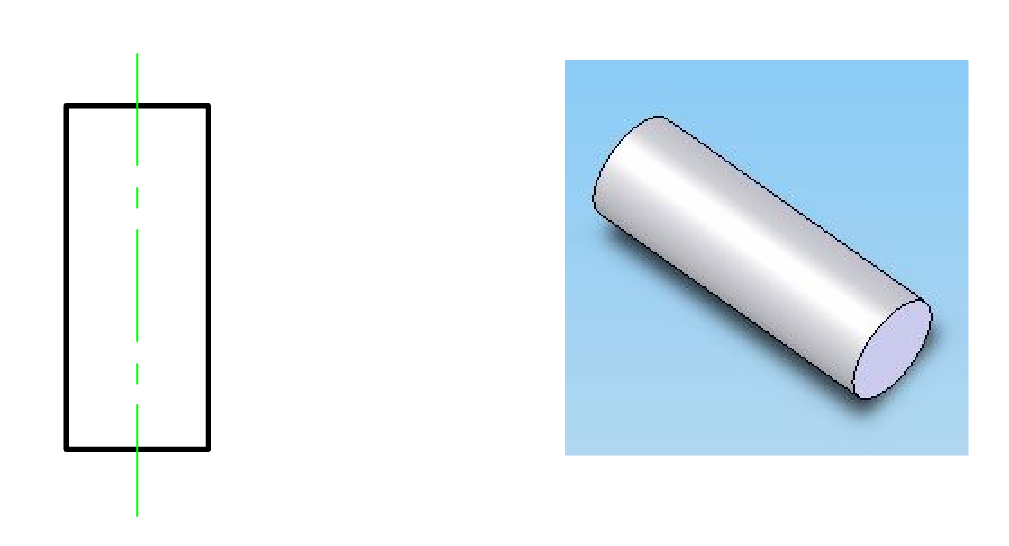
\includegraphics[width = 8 cm]{Images/ImagesDessinTechnique/axeRevolution.png}
    \caption{Utilisation de l'axe mixte dans la représentation d'un cylindre. Aucune autre vue n'est nécessaire.}
    \label{fig:my_label}
\end{figure}


\subsection{Représentation des arêtes}
Dans un plan, il faut représenter \textbf{toutes} les arêtes visibles dans cette vue.

\begin{figure}[H]
    \centering
    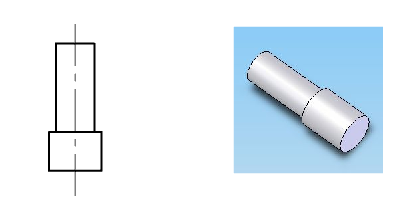
\includegraphics[width = 8cm]{Images/ImagesDessinTechnique/AretesCylindre.png}
    \caption{Représentation d'un cylindre à section variable. Il ne faut pas oublier l'arête faisant la délimitation entre les deux "parties"}
    \label{fig:my_label}
\end{figure}

Si l'on décide d'ajouter un plat au cylindre comme suit, on doit alors 
\begin{enumerate}
    \item Ajouter les nouvelles arêtes visibles sur le dessin
    \item Ajouter une seconde vue. En effet, l'unique vue précédente ne permet pas d'indiquer la "profondeur du plat".
\end{enumerate}

\begin{figure}[H]
    \centering
    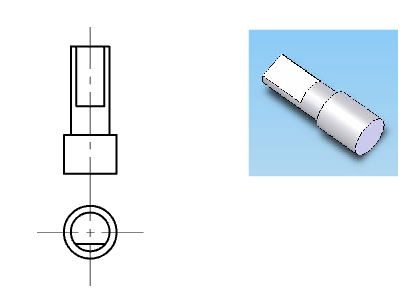
\includegraphics[width = 8cm]{Images/ImagesDessinTechnique/platCylindre.png}
    \caption{Ajout d'un plat au solide précédent}
    \label{fig:cylindrePlat}
\end{figure}



\subsection{Perçage de trous}

Si l'on souhaite percer un trou dans le plat du cylindre dessiné dans la figure \ref{fig:cylindrePlat}, il suffit d'ajouter sur la vue de face, un \textbf{cercle} ainsi que \textbf{son trait d'axe}.\\
Sans information supplémentaires, on considérera que le trou est traversant.\\

Il est également possible d'ajouter sur la vue du dessus la profondeur du trou. Cela doit se faire en trait discontinus car les arêtes sont cachées.

\begin{figure}[H]
    \centering
    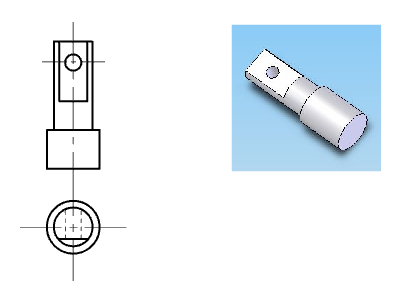
\includegraphics[width = 8cm]{Images/ImagesDessinTechnique/trouCylindre.png}
    \caption{Ajout d'un trou dans le solide.}
    \label{fig:my_label}
\end{figure}

Pour représenter un trou borgne, il faut alors rajouter les arêtes cachées dans la vue principale.\\
Un trou est percé avec un foret. Le bout d'un foret est pointu. Il ne faut donc pas oublier de rajouter la pointe dans le trous.

\begin{figure}[H]
    \centering
    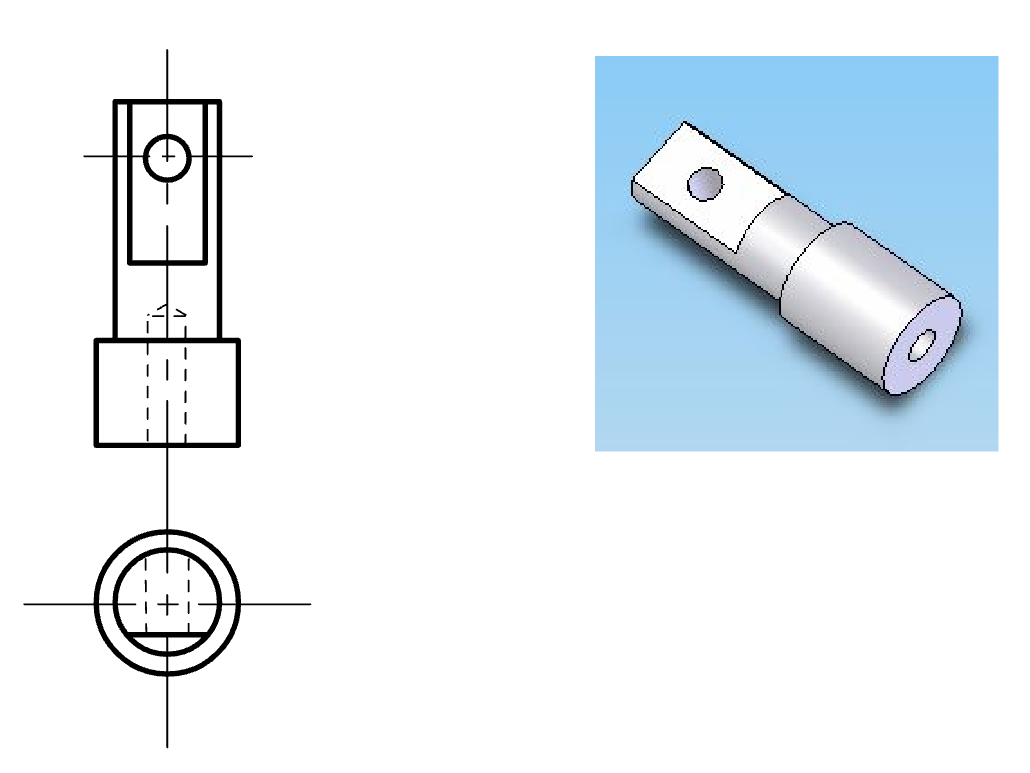
\includegraphics[width = 8cm]{Images/ImagesDessinTechnique/foretCyclindre.png}
    \caption{Perçage d'un trou borgne avec un foret}
    \label{fig:foret}
\end{figure}


%Est-ce qu'on ne s'en fiche pas un peu tout compte fait ?
%\chapter{Les moteurs à combustion interne}
%\textcolor{green}{Je suis à moitié en freestyle, à moitié en train de traduire le texte, donc il y aura sans doute beaucoup à corriger. (Julien Monfils)}

\section{Gudgeon pin \textcolor{red}{J'ai pas la traduction}}
\textcolor{red}{TODO, j'ai pas compris}

%J'ai skip 12.5 "Journal bearing load considerations" car la section n'est pas complète dans le pdf des extraits.

\section{Propriétés du matériau souhaitées pour la fabrication du bloc-moteur}
On souhaite que le matériau utilisé ai les propriétés suivantes :
\begin{itemize}
    \item Il doit être relativement peu cher
    \item Il doit pouvoir être moulé
    \item Il doit être facilement usiné
    \item Il doit être assez résistant, autant en torsion qu'en \textcolor{red}{bending => pliage ? Flambage ? Je ne trouve pas de traduction}
    \item Il doit être résistant à l'abrasion et à la corrosion
    \item Il doit avoir une dillatation thermique faible \textcolor{red}{Pas sûr de la traduction}
    \item Il doit avoir une conductivité thermique élevée
    \item Il être assez résistant à hautes températures
    \item Il doit avoir une densité relativement faible
\end{itemize}
\\

On remarque que la fonte correspond à la plus part des critères. Néanmoins, la fonte a une conductivité thermique très faible. C'est pourquoi on peut également utiliser un alliage d'aluminium léger. Il faut cependant faire attention, l'alliage d'aluminium est moins résistant à l'usure que la fonte, c'est pourquoi il faut augmenter la section du moulage \textcolor{red}{"and additional support ribs", je ne sais pas comment le traduire}. Ce qui augmente considérablement la masse du bloc-moteur en alliage.\\
De manière générale, un bloc en fonte a un masse deux fois plus élevée que celle d'un bloc en alliage d'aluminium léger.

\section{Le piston}
\begin{figure}[H]
    \centering
    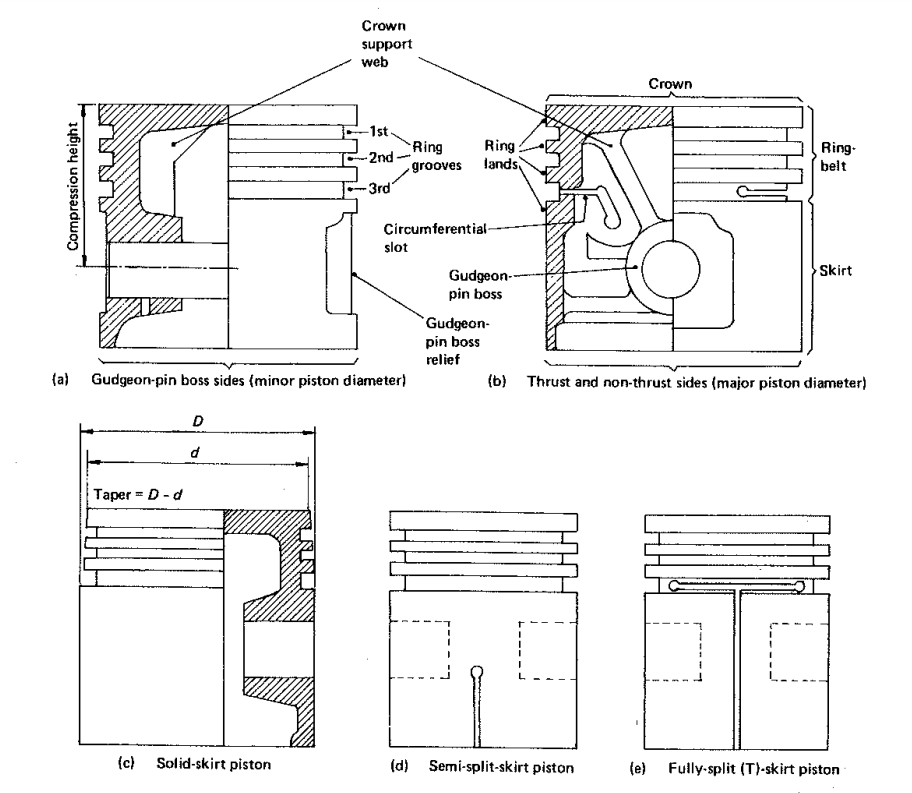
\includegraphics[width = 15cm]{Images/ImagesICE/PistonNomenclature.png}
    \caption{Fluctuation de la masse volumique en fonction du volume de l'élément \protect \footnotemark}
    \label{fig:fluctuationsVER}
\end{figure}
\footnotetext{Vehicle and engine technology, Heisler Heinz}

\textcolor{red}{TODO}

\end{document}